\documentclass[12pt]{article}

\usepackage{report}

\usepackage[utf8]{inputenc} % allow utf-8 input
\usepackage[T1]{fontenc}    % use 8-bit T1 fonts
\usepackage[colorlinks=true, linkcolor=black, citecolor=blue, urlcolor=blue]{hyperref}       % hyperlinks
\usepackage{url}            % simple URL typesetting
\usepackage{booktabs}       % professional-quality tables
\usepackage{amsfonts}       % blackboard math symbols
\usepackage{nicefrac}       % compact symbols for 1/2, etc.
\usepackage{microtype}      % microtypography
\usepackage{lipsum}		% Can be removed after putting your text content
\usepackage{graphicx}
\usepackage{natbib}
\usepackage{doi}
\usepackage{listings}
\usepackage{xcolor}
\usepackage{float}
\setcitestyle{aysep={,}}



\title{Project Step 1}

\author{Ulises Espinoza-Gonzalez and Jack Stolpman\\
\AND\\
\AND
\AND
\AND
\AND
	CS.3339 Computer Architecture\\
\AND
	Texas State University\\
}

% Uncomment to remove the date
\date{September 26, 2024}

% Uncomment to override  the `A preprint' in the header
\renewcommand{\headeright}{Project Step 1 - Tomato}
\renewcommand{\undertitle}{Group Tomato}
\renewcommand{\shorttitle}{}

\definecolor{codegreen}{rgb}{0,0.6,0}
\definecolor{codegray}{rgb}{0.5,0.5,0.5}
\definecolor{codepurple}{rgb}{0.58,0,0.82}
\definecolor{backcolour}{rgb}{0.95,0.95,0.92}

\lstdefinestyle{mystyle}{
    backgroundcolor=\color{backcolour},   
    commentstyle=\color{codegreen},
    keywordstyle=\color{magenta},
    numberstyle=\tiny\color{codegray},
    stringstyle=\color{codepurple},
    basicstyle=\ttfamily\footnotesize,
    breakatwhitespace=false,         
    breaklines=true,                 
    captionpos=b,                    
    keepspaces=true,                 
    numbers=left,                    
    numbersep=5pt,                  
    showspaces=false,                
    showstringspaces=false,
    showtabs=false,                  
    tabsize=2
}

\lstset{style=mystyle}


\begin{document}
\maketitle

\newpage
%\tableofcontents
\thispagestyle{empty}


\newpage
\setcounter{page}{1}
\section{Introduction}
Digital logic and circuits are an essential part of understanding the hardware components of any electronic device. Hardware descriptive languages such as Verilog, introduce us to the process of designing a new computer circuit from scratch. In this first section of our project, we will be utilizing 1-bit Not, Nand, Nor, and 1x4-bit input / 1x4-bit output shift circuits to generate simulation waveforms. Some goals that we as a group share is to improve our understanding of the methodology of designing new computer circuits from scratch. We also wish to familiarize ourselves with the Verilog programming language, which is new to us. 

\section{Verilog Code}
\label{sec:headings}

In this section, we are going to go over the circuits and then the Verilog code for each one with the test modules.






\section{Not Circuit}
The Not circuit takes two inputs: A and B.The Not gate will revert the value inputted. If the value of A is 1, then the value of B will be 0 and vice versa.
\lstinputlisting[language=Verilog]{Verilog/NotCompArchFirst_tb.v}

To test the Not circuit, we have created two registers, A and B. This way we can take two inputs at a time and test each possible input for the circuit. If it's working correctly, A should be equal to 1 whenever B is equal to 0.
\lstinputlisting[language=Verilog]{Verilog/NotCompArchFirst.v}

\begin{figure}[h]
    \centering
    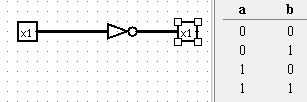
\includegraphics[width = 1.0\textwidth]{figs/Not CircuitTruth.png}
    \caption{Not truth table and gate}
    \label{fig:enter-label}
\end{figure}

\newpage



\subsection{Waveform Tests}

The last section we will showcase the waveforms created using our testbenches for each circuit we coded in Verilog. We used GTKWave to create these waveforms.



\section{Nand Circuit}
The Nand circuit takes two inputs, A and B, with an output X. This output will only shoot back a 1 assuming that both A and B are not equal to 1, hence the Nand (Not and) logic gate
\lstinputlisting[language=Verilog]{Verilog/NandCompArchFirst_tb.v}

To test the Nand circuit, we have created two registers, A and B, as well as a wire X. This way we are able to take two inputs at a time and test each possible input for the circuit. If it's working correctly, X should be equal to 1 for all inputs except when both A and B are equal to 1
\lstinputlisting[language=Verilog]{Verilog/NandCompArchFirst.v}

\begin{figure}[h]
    \centering
    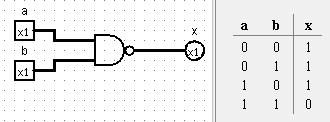
\includegraphics[width = 1.0\textwidth]{figs/Nand CircuitTruth.png}
    \caption{Nand truth table and gate}
    \label{fig:enter-label}
\end{figure}

\newpage

\subsection{Waveform Tests}

The last section we will showcase the waveforms created using our testbenches for each circuit we coded in Verilog. We used GTKWave to create these waveforms.







\section{Nor Circuit}
The Nor circuit takes two inputs, A and B, with an output X. This output will only shoot back a 1 assuming that both A and B are equal to 0, hence the Nor logic gate. For the output to return a high value, both inputs need to be low.
\lstinputlisting[language=Verilog]{Verilog/NorCompArchFirst_tb.v}

To test the Nor circuit, we have created two registers, A and B, as well as a wire X. This way we are able to take two inputs at a time and test each possible input for the circuit. If it's working correctly, X should be equal to 1 for all inputs except when both A and B are equal to 0. 
\lstinputlisting[language=Verilog]{Verilog/NorCompArchFirst.v}

\begin{figure}[h]
    \centering
    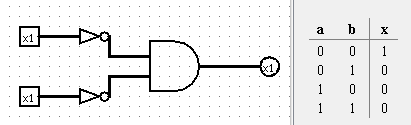
\includegraphics[width = 1.0\textwidth]{figs/Nor CircuitTruth.png}
    \caption{Nor truth table and gate}
    \label{fig:enter-label}
\end{figure}

\newpage

\subsection{Waveform Tests}

The last section we will showcase the waveforms created using our testbenches for each circuit we coded in Verilog. We used GTKWave to create these waveforms.





\section{1x4-bit input Circuit}
The 4 bit input circuit takes two inputs, fourin and fourout. We create a shift input 
\lstinputlisting[language=Verilog]{Verilog/InputCompArchFirst_tb.v}
To test this 4 bit circuit, we create a register that takes in a 4 bit value. This value works alongside the clock which when executed using the @posedge and the clock signal goes from high to low, the input will be transfered into the output.

\lstinputlisting[language=Verilog]{Verilog/InputCompArchFirst.v}



\subsection{Waveform Tests}

The last section we will showcase the waveforms created using our testbenches for each circuit we coded in Verilog. We used GTKWave to create these waveforms.






\section{1x4-bit output Shift Circuit}
The 4 bit input circuit takes two inputs, datain and dataout. We use a clock/ reset and create a shift input in order to determine the shift direction (high = 1 = right, low = 0 = left).  On the rising edge of the reset, we set the output to 4'b0000 (0 in verilog) which clears the shift register. While this process is happening, if the shift is high, the data is shifted right by 1 bit and when the shift is low, the data is shifted left by 1 bit.

\lstinputlisting[language=Verilog]{Verilog/ShiftCompArchFirst_tb.v}

To test the 4bit shift circuit, we have created two registers, A and B, as well as a wire X. We also create a 
\lstinputlisting[language=Verilog]{Verilog/ShiftCompArchFirst.v}



\subsection{Waveform Tests}

The last section we will showcase the waveforms created using our testbenches for each circuit we coded in Verilog. We used GTKWave to create these waveforms.


\section{Conclusion}

In conclusion, we successfully created and tested various circuits using Verilog and GTKWave. Learning how to code in Verilog, at least for our purposes, was relatively simple with few difficulties. Using GTKWave was also fairly intuitive. The most difficulty our group has had so far was most likely creating this report in LaTeX, as we have some trouble with coding certain formatting as well as issues with figures floating around the document. Creating these logic circuits from scratch allowed us to work on the basic logic gates (NOT, NAND, NOR) that are so critical to all electronics. The use of Verilog and GTKWave works as a stepping stone to furthering our engineering careers and building on our knowledge of both the software and hardware components of electronics.




\section{Waveforms}


\subsection{Not Circuit Waveform}

At 0 ns, we can see that both A and B are 0, so the output X is 1 which is consistent with the NOT gate.
\begin{figure}[h]
    \centering
    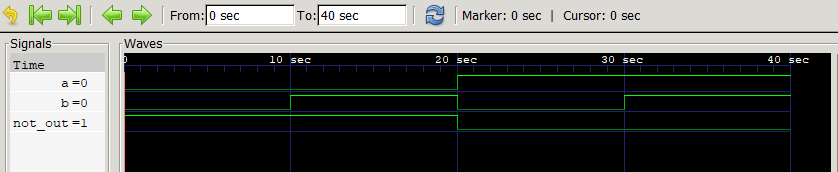
\includegraphics[width = 1.0\textwidth]{figs/Not0.png}
    \caption{Not Circuit with marker at 0ns}
    \label{fig:enter-label}
\end{figure}


At 20 ns, A is 1 and B is 0, so X is 0
\begin{figure}[h]
    \centering
    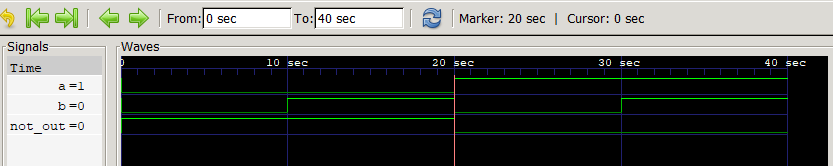
\includegraphics[width = 1.0\textwidth]{figs/Not20.png}
    \caption{Not Circuit with marker at 20ns}
    \label{fig:enter-label}
\end{figure}

\newpage

At 40 ns, both A and B are 1, so X is now 0 because the not condition has been upheld
\begin{figure}[h]
    \centering
    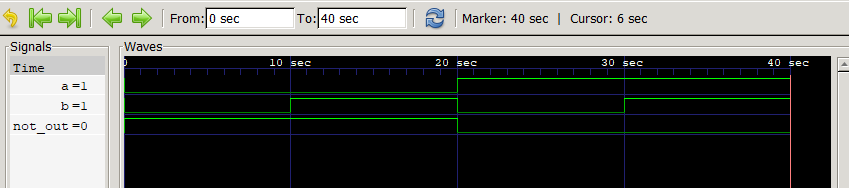
\includegraphics[width = 1.0\textwidth]{figs/Not40.png}
    \caption{Not Circuit with marker at 40ns}
    \label{fig:enter-label}
\end{figure}



\subsection{Nand Circuit Waveform}

At 0 ns, we can see that both A and B are 0, so the output X is 1 which is consistent with Nand gate behavior where both inputs have to be high(1) for the output to become low(0).
\begin{figure}[h]
    \centering
    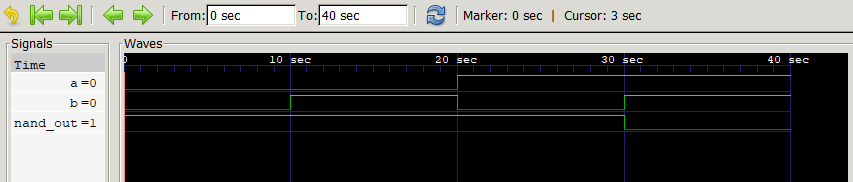
\includegraphics[width = 1.0\textwidth]{figs/Nand0.png}
    \caption{Nand Circuit with marker at 0ns}
    \label{fig:enter-label}
\end{figure}

At 10 ns, A is 0 and B is 1, so X still remains at 1
\begin{figure}[h]
    \centering
    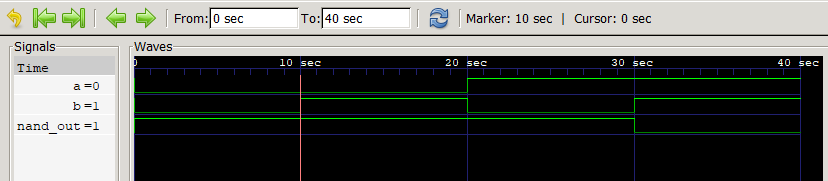
\includegraphics[width = 1.0\textwidth]{figs/nand10.png}
    \caption{Nand Circuit with marker at 10ns}
    \label{fig:enter-label}
\end{figure}

\newpage

At 20 ns, A is 1 and B is 0, so X still remains at 1
\begin{figure}[h]
    \centering
    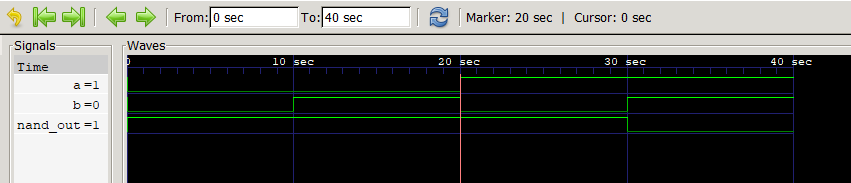
\includegraphics[width = 1.0\textwidth]{figs/Nand20.png}
    \caption{Nand Circuit with marker at 20ns}
    \label{fig:enter-label}
\end{figure}


At 30 ns, A is 1 and B is 1, so X is 0
\begin{figure}[h]
    \centering
    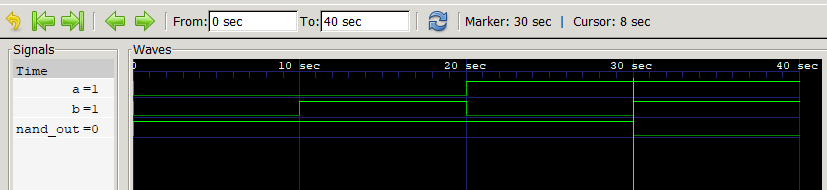
\includegraphics[width = 1.0\textwidth]{figs/Nand30.png}
    \caption{Nand Circuit with marker at 30ns}
    \label{fig:enter-label}
\end{figure}

At 40 ns, both A and B are 1, so X is now 0 because the Nand gate requires both inputs to be  high(1) in order for the output to become low (0).
\begin{figure}[h]
    \centering
    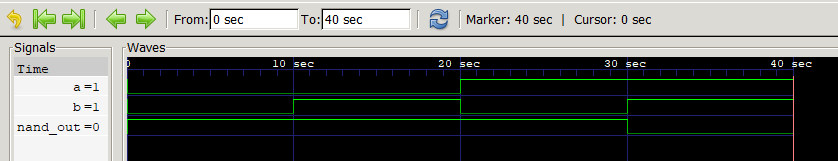
\includegraphics[width = 1.0\textwidth]{figs/Nand40.png}
    \caption{Nand Circuit with marker at 40ns}
    \label{fig:enter-label}
\end{figure}

\newpage

\subsection{Nor Circuit Waveform}

At 0 ns, we can see that both A and B are 0, so the output X is 1
\begin{figure}[h]
    \centering
    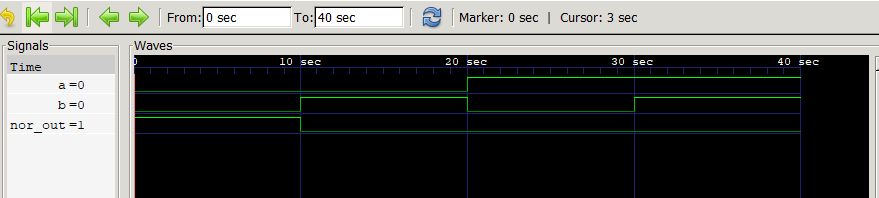
\includegraphics[width = 1.0\textwidth]{figs/Nor0.png}
    \caption{Nor Circuit with marker at 0ns}
    \label{fig:enter-label}
\end{figure}


At 10 ns, we can see that A is 0 and B is 1, so the output X is 0
\begin{figure}[h]
    \centering
    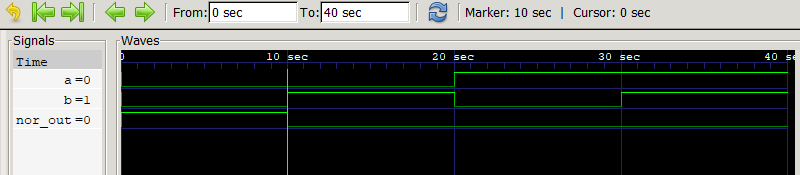
\includegraphics[width = 1.0\textwidth]{figs/Nor10.png}
    \caption{Nor Circuit with marker at 10ns}
    \label{fig:enter-label}
\end{figure}

At 20 ns, A is 1 and B is 0, so X is 1
\begin{figure}[h]
    \centering
    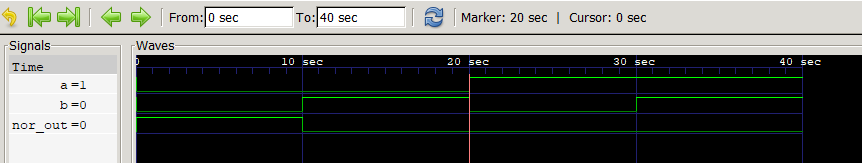
\includegraphics[width = 1.0\textwidth]{figs/Nor20.png}
    \caption{Nor Circuit with marker at 20ns}
    \label{fig:enter-label}
\end{figure}

\newpage

At 30 ns, A is 1 and B is 1, so X is 0
\begin{figure}[h]
    \centering
    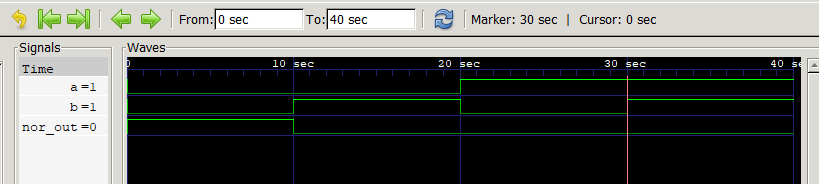
\includegraphics[width = 1.0\textwidth]{figs/Nor30.png}
    \caption{Nor Circuit with marker at 30ns}
    \label{fig:enter-label}
\end{figure}


At 40 ns, both A and B are 1, so X is now 0 
\begin{figure}[h]
    \centering
    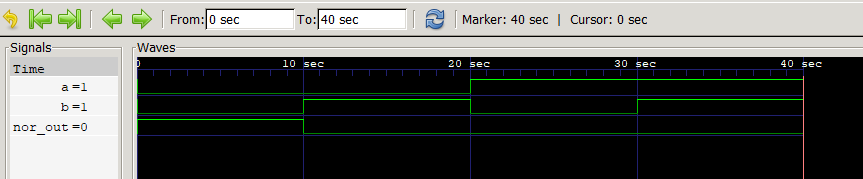
\includegraphics[width = 1.0\textwidth]{figs/Nor40.png}
    \caption{Nor Circuit with marker at 40ns}
    \label{fig:enter-label}
\end{figure}




\subsection{1x4-bit input Circuit Waveform}

At 0 s, we can see that four in is 0, so the output four out is 0
\begin{figure}[h]
    \centering
    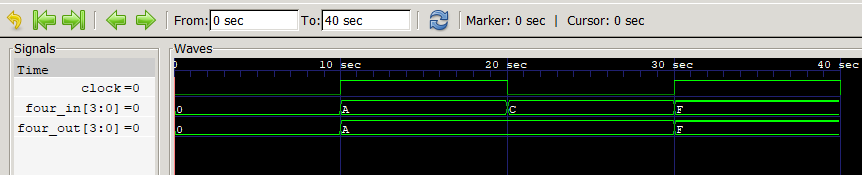
\includegraphics[width = 1.0\textwidth]{figs/Input0.png}
    \caption{1x4-bit input Circuit with marker at 0ns}
    \label{fig:enter-label}
\end{figure}

\newpage

At 10 s, we can see that four in is A, so the output four out is A
\begin{figure}[h]
    \centering
    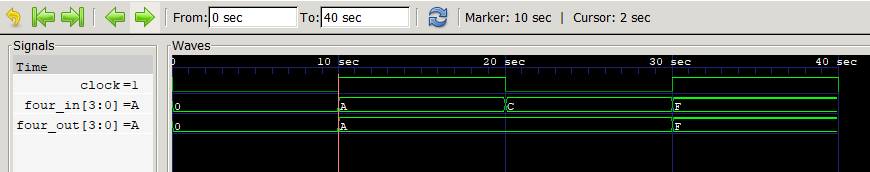
\includegraphics[width = 1.0\textwidth]{figs/Input10.png}
    \caption{1x4-bit input Circuit with marker at 10ns}
    \label{fig:enter-label}
\end{figure}


At 20 s, four in is C, so four out is A
\begin{figure}[h]
    \centering
    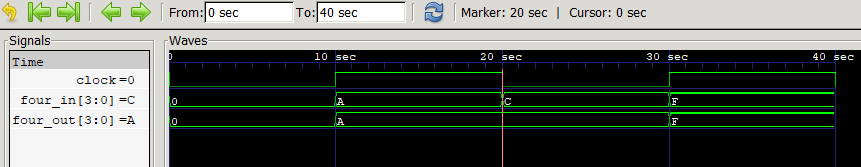
\includegraphics[width = 1.0\textwidth]{figs/Input20.png}
    \caption{1x4-bit input Circuit with marker at 20ns}
    \label{fig:enter-label}
\end{figure}

At 30 s, four in is F, so four out is F
\begin{figure}[h]
    \centering
    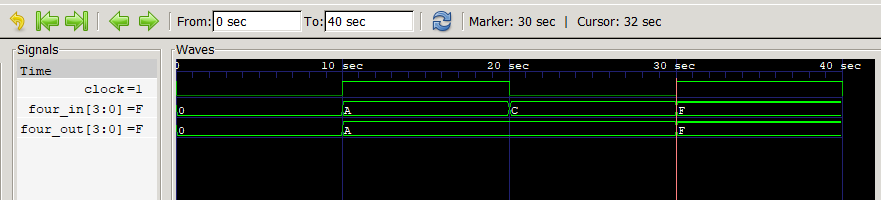
\includegraphics[width = 1.0\textwidth]{figs/Input30.png}
    \caption{1x4-bit input Circuit with marker at 30ns}
    \label{fig:enter-label}
\end{figure}

\newpage

At 40 s, four in is F and four out becomes F
\begin{figure}[h]
    \centering
    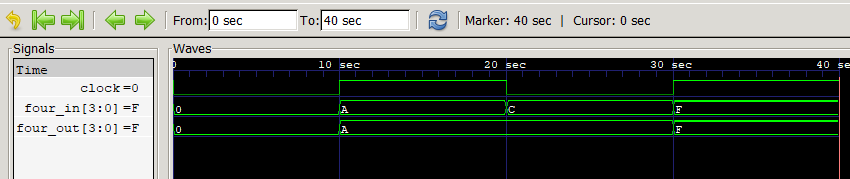
\includegraphics[width = 1.0\textwidth]{figs/Input40.png}
    \caption{1x4-bit input Circuit with marker at 40ns}
    \label{fig:enter-label}
\end{figure}


\subsection{1x4-bit output Shift Circuit Waveform}

At 0 s, we can see that four in is 0, four shifted is 0 and right shift is 0
\begin{figure}[h]
    \centering
    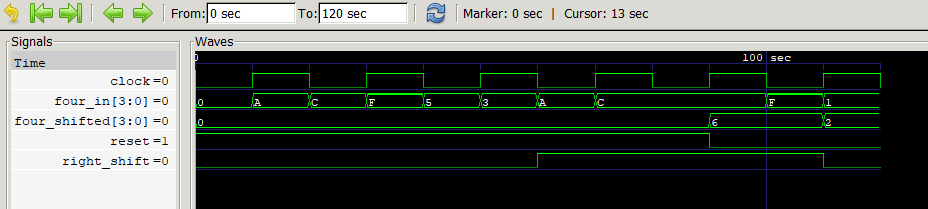
\includegraphics[width = 1.0\textwidth]{figs/Shift0.png}
    \caption{1x4-bit output Shift Circuit with marker at 0s}
    \label{fig:enter-label}
\end{figure}

At 10 s, we can see that four in is A, four shifted is 0 and right shift is 0
\begin{figure}[h]
    \centering
    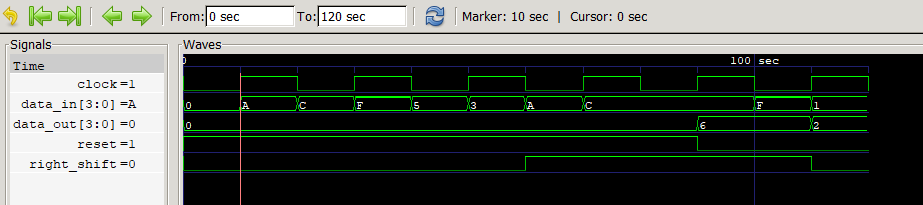
\includegraphics[width = 1.0\textwidth]{figs/Shift10.png}
    \caption{1x4-bit output Shift Circuit with marker at 10s}
    \label{fig:enter-label}
\end{figure}

\newpage

At 20 s, we can see that four in is C, four shifted is 0 and right shift is 0
\begin{figure}[h]
    \centering
    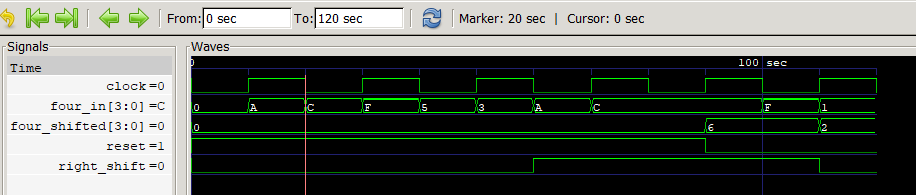
\includegraphics[width = 1.0\textwidth]{figs/Shift20.png}
    \caption{1x4-bit output Shift Circuit with marker at 20s}
    \label{fig:enter-label}
\end{figure}

At 30 s, we can see that four in is F, four shifted is 0 and right shift is 0
\begin{figure}[h]
    \centering
    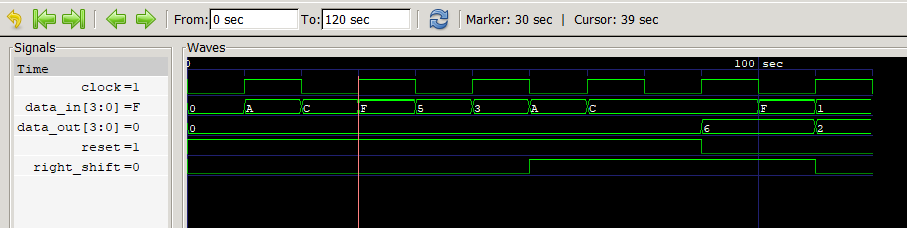
\includegraphics[width = 1.0\textwidth]{figs/Shift30.png}
    \caption{1x4-bit output Shift Circuit with marker at 30s}
    \label{fig:enter-label}
\end{figure}

At 40 s, four in is 5, four shifted is 0 and right shift is 0
\begin{figure}[h]
    \centering
    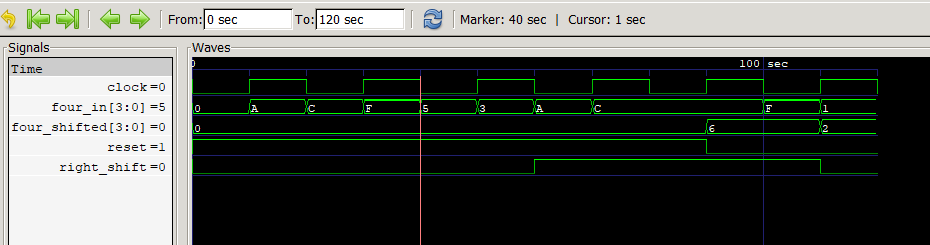
\includegraphics[width = 1.0\textwidth]{figs/Shift40.png}
    \caption{1x4-bit output Shift Circuit with marker at 40s}
    \label{fig:enter-label}
\end{figure}

\newpage

At 50 s, we can see that four in is 3, four shifted is 0 and right shift is 0
\begin{figure}[h]
    \centering
    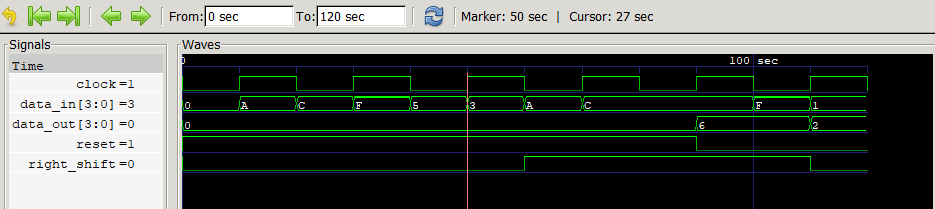
\includegraphics[width = 1.0\textwidth]{figs/Shift50.png}
    \caption{1x4-bit output Shift Circuit with marker at 50s}
    \label{fig:enter-label}
\end{figure}

At 60 s, we can see that four in is A, four shifted is 0 and right shift is 1
\begin{figure}[h]
    \centering
    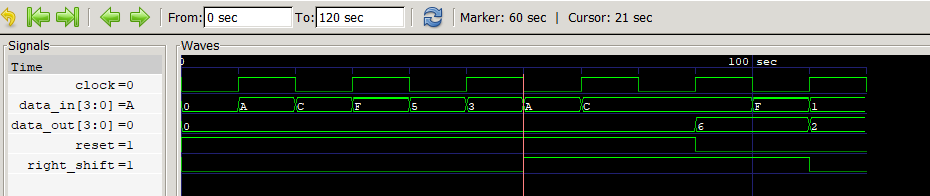
\includegraphics[width = 1.0\textwidth]{figs/Shift60.png}
    \caption{1x4-bit output Shift Circuit with marker at 60s}
    \label{fig:enter-label}
\end{figure}

At 70 s, we can see that four in is C, four shifted is 0 and right shift is 1
\begin{figure}[h]
    \centering
    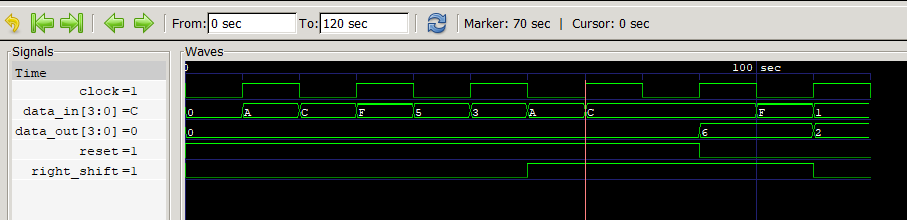
\includegraphics[width = 1.0\textwidth]{figs/Shift70.png}
    \caption{1x4-bit output Shift Circuit with marker at 70s}
    \label{fig:enter-label}
\end{figure}

\newpage

At 80 s, we can see that four in is C, four shifted is 0 and right shift is 1
\begin{figure}[h]
    \centering
    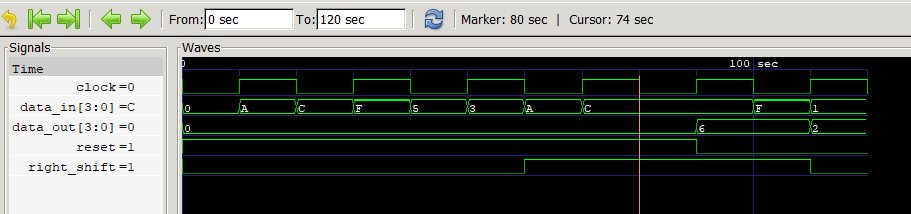
\includegraphics[width = 1.0\textwidth]{figs/Shift80.png}
    \caption{1x4-bit output Shift Circuit with marker at 80s}
    \label{fig:enter-label}
\end{figure}

At 90 s, we can see that four in is C, four shifted is 6 and right shift is 1
\begin{figure}[h]
    \centering
    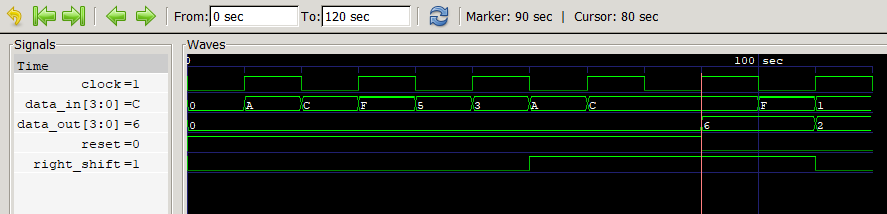
\includegraphics[width = 1.0\textwidth]{figs/Shift90.png}
    \caption{1x4-bit output Shift Circuit with marker at 90s}
    \label{fig:enter-label}
\end{figure}

At 100 s, we can see that four in is F, four shifted is 6 and right shift is 1
\begin{figure}[h]
    \centering
    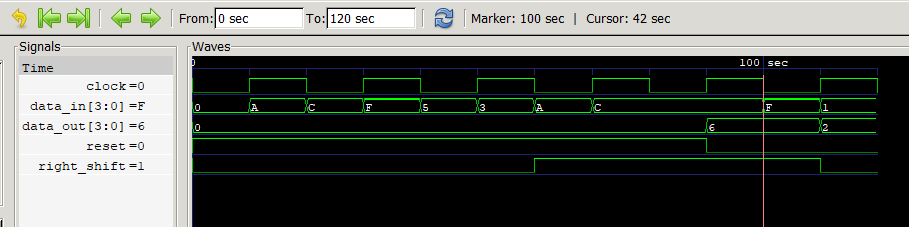
\includegraphics[width = 1.0\textwidth]{figs/Shift100.png}
    \caption{1x4-bit output Shift Circuit with marker at 100s}
    \label{fig:enter-label}
\end{figure}

\newpage

At 110 s, we can see that four in is 1, four shifted is 2 and right shift is 0
\begin{figure}[h]
    \centering
    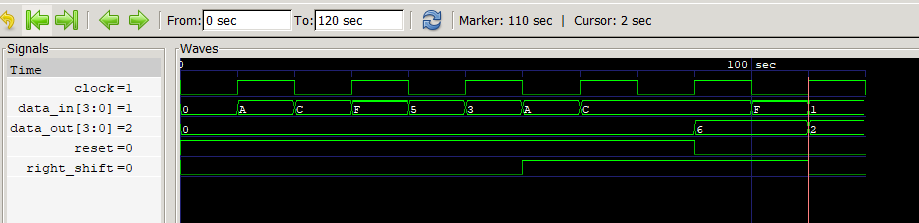
\includegraphics[width = 1.0\textwidth]{figs/Shift110.png}
    \caption{1x4-bit output Shift Circuit with marker at 110s}
    \label{fig:enter-label}
\end{figure}

At 120 s, we can see that four in is 1, four shifted is 2 and right shift is 0
\begin{figure}[h]
    \centering
    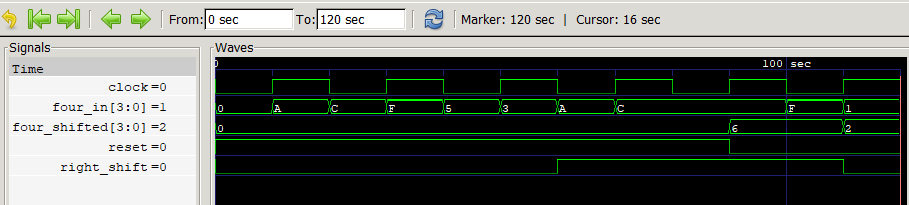
\includegraphics[width = 1.0\textwidth]{figs/Shift120.png}
    \caption{1x4-bit output Shift Circuit with marker at 120s}
    \label{fig:enter-label}
\end{figure}




\end{document}